\chapter{Electron Shells and the Periodic Table}\label{ch:g10:electron-shells}

Neon glows red-orange in a sign; sodium, a soft \omterm{def:g9:periodic-table-first-look:metal}{metal}, catches fire in
water; chlorine is a choking yellow-green gas. Yet their \omterm{def:g7:atoms-and-molecules:atom}{atoms} differ by
only one or two \omterm{def:g9:inside-the-atom:proton}{protons}: neon has 10, sodium 11, chlorine 17. Why should
neighbours in the \omterm{def:g9:periodic-table-first-look:periodic-table}{periodic table} behave so differently, while sodium and
potassium, far apart in \omterm{def:g9:inside-the-atom:atomic-number}{atomic number}, behave so alike? The answer lies
in how the \omterm{def:g9:inside-the-atom:nucleus}{electrons} of an \omterm{def:g7:atoms-and-molecules:atom}{atom} are arranged.

\begin{recall}
An \omterm{def:g7:atoms-and-molecules:atom}{atom} has $Z$ \omterm{def:g9:inside-the-atom:proton}{protons} in its \omterm{def:g9:inside-the-atom:nucleus}{nucleus} and, when neutral, $Z$ \omterm{def:g9:inside-the-atom:nucleus}{electrons}
around it (\cref{ch:g9:inside-the-atom}). The \omterm{def:g9:periodic-table-first-look:periodic-table}{periodic table} orders the
elements by $Z$ in periods (rows) and groups (columns); elements of a
group behave alike (\cref{ch:g9:periodic-table-first-look}). \omterm{def:g7:atoms-and-molecules:atom}{Atoms} gain or
lose \omterm{def:g9:inside-the-atom:nucleus}{electrons} to become \omterm{def:g9:ions:ion}{ions} (\cref{ch:g9:ions}).
\end{recall}

\section{Electron configuration}

\begin{definition}[Shells, subshells and electron configuration]\label{def:g10:electron-shells:configuration}
The \omterm{def:g9:inside-the-atom:nucleus}{electrons} of an \omterm{def:g7:atoms-and-molecules:atom}{atom} are arranged in \emph{shells}\index{shell},
numbered $n = 1, 2, 3, \ldots$ from the \omterm{def:g9:inside-the-atom:nucleus}{nucleus} outwards; the higher
$n$, the further from the \omterm{def:g9:inside-the-atom:nucleus}{nucleus} and the less tightly held the
\omterm{def:g9:inside-the-atom:nucleus}{electrons}. Each shell is divided into \emph{subshells}\index{subshell}
named by a letter: shell 1 has an s subshell (1s), shell 2 an s and a p
subshell (2s, 2p), shell 3 has 3s and 3p (and 3d, met later). An s
subshell holds at most 2 \omterm{def:g9:inside-the-atom:nucleus}{electrons}, a p subshell at most 6. The
\emph{electron configuration}\index{electron configuration} of an \omterm{def:g7:atoms-and-molecules:atom}{atom}
lists its occupied subshells with their numbers of \omterm{def:g9:inside-the-atom:nucleus}{electrons} as
exponents: $1\mathrm{s}^2\,2\mathrm{s}^2\,2\mathrm{p}^4$ for oxygen.
\end{definition}

\begin{method}[Writing an electron configuration, up to $Z = 20$]\label{met:g10:electron-shells:write}
\begin{enumerate}
  \item Count the \omterm{def:g9:inside-the-atom:nucleus}{electrons}: $Z$ for a neutral \omterm{def:g7:atoms-and-molecules:atom}{atom}.
  \item Fill the \omterm{def:g10:electron-shells:configuration}{subshells} in this order, each up to its maximum before
        starting the next:
        \[
          1\mathrm{s} \to 2\mathrm{s} \to 2\mathrm{p} \to 3\mathrm{s} \to
          3\mathrm{p} \to 4\mathrm{s}.
        \]
  \item Check that the exponents add up to the number of \omterm{def:g9:inside-the-atom:nucleus}{electrons}.
\end{enumerate}
Sodium, $Z = 11$: $1\mathrm{s}^2\,2\mathrm{s}^2\,2\mathrm{p}^6\,3\mathrm{s}^1$.
Chlorine, $Z = 17$: $1\mathrm{s}^2\,2\mathrm{s}^2\,2\mathrm{p}^6\,3\mathrm{s}^2\,3\mathrm{p}^5$.
Calcium, $Z = 20$: $1\mathrm{s}^2\,2\mathrm{s}^2\,2\mathrm{p}^6\,3\mathrm{s}^2\,3\mathrm{p}^6\,4\mathrm{s}^2$.
\end{method}

\begin{omfigure}
\begin{tikzpicture}[font=\small, y=0.95cm]
  \draw[->, black!60] (-0.4,0) -- (-0.4,5.4) node[above, align=center, font=\footnotesize]
    {further from\\ the nucleus};
  \foreach \y/\lab/\n/\x in {0.3/1s/2/0.5, 1.3/2s/2/0.5, 1.9/2p/6/2.4, 3.0/3s/2/0.5,
      3.6/3p/6/2.4, 4.4/4s/2/0.5} {
    \foreach \k in {1,...,\n} \draw[omDef, fill=omDef!10] (\x+0.42*\k-0.42,\y) rectangle ++(0.36,0.36);
    \node[anchor=east] at (\x-0.05,\y+0.18) {\lab};
  }
  \node[anchor=west, font=\footnotesize] at (5.3,0.48) {shell 1: 2 electrons at most};
  \node[anchor=west, font=\footnotesize] at (5.3,1.7) {shell 2: $2 + 6 = 8$};
  \node[anchor=west, font=\footnotesize] at (5.3,3.4) {shell 3: $2 + 6 = 8$ (up to $Z = 18$)};
  \node[anchor=west, font=\footnotesize] at (5.3,4.58) {4s fills before 3d};
\end{tikzpicture}

{\small The order of filling, up to $Z = 20$. Each small box is a place
for one \omterm{def:g9:inside-the-atom:nucleus}{electron}: an s \omterm{def:g10:electron-shells:configuration}{subshell} has 2 places, a p \omterm{def:g10:electron-shells:configuration}{subshell} 6.}
\end{omfigure}

\section{Valence electrons}

\begin{definition}[Valence and core electrons]\label{def:g10:electron-shells:valence}
The \omterm{def:g9:inside-the-atom:nucleus}{electrons} of the outermost occupied \omterm{def:g10:electron-shells:configuration}{shell} (the \omterm{def:g10:electron-shells:configuration}{shell} with the
highest $n$) are the \emph{valence electrons}\index{valence electron};
the others are the \emph{core electrons}\index{core electron}. Only the
valence \omterm{def:g9:inside-the-atom:nucleus}{electrons} take part in \omterm{def:g7:chemical-reactions:reaction}{chemical reactions}.
\end{definition}

\begin{example}[Counting valence electrons]\label{ex:g10:electron-shells:count}
Oxygen, $1\mathrm{s}^2\,2\mathrm{s}^2\,2\mathrm{p}^4$: outer \omterm{def:g10:electron-shells:configuration}{shell} $n =
2$, $2 + 4 = 6$ \omterm{def:g10:electron-shells:valence}{valence electrons}. Sodium, $\ldots 3\mathrm{s}^1$: 1
\omterm{def:g10:electron-shells:valence}{valence electron}. Chlorine, $\ldots 3\mathrm{s}^2\,3\mathrm{p}^5$: 7.
Neon, $1\mathrm{s}^2\,2\mathrm{s}^2\,2\mathrm{p}^6$: 8, a full \omterm{def:g10:electron-shells:configuration}{shell}.
\end{example}

\section{The table rebuilt from configurations}

\begin{proposition}[Period and group from the configuration]\label{prop:g10:electron-shells:table}
For the elements up to $Z = 20$:
\begin{itemize}
  \item the period of an element is the number $n$ of its outer \omterm{def:g10:electron-shells:configuration}{shell};
  \item elements of a same group have the same number of \omterm{def:g10:electron-shells:valence}{valence
        electrons} --- one in \omterm{def:g9:periodic-table-first-look:period}{group} 1, two in \omterm{def:g9:periodic-table-first-look:period}{group} 2, three to eight in
        \omterm{def:g9:periodic-table-first-look:period}{groups} 13 to 18 (helium, with 2, is an exception).
\end{itemize}
The left two columns, where the last \omterm{def:g9:inside-the-atom:nucleus}{electrons} enter an s \omterm{def:g10:electron-shells:configuration}{subshell}, form
the s block; \omterm{def:g9:periodic-table-first-look:period}{groups} 13 to 18 form the p block.
\end{proposition}

\begin{omfigure}
\omperiodictable[upto=20, f block=false, cell=0.86cm, colour=blocks, legend=true,
  values={H/1,He/2,Li/2.1,Be/2.2,B/2.3,C/2.4,N/2.5,O/2.6,F/2.7,Ne/2.8,
    Na/2.8.1,Mg/2.8.2,Al/2.8.3,Si/2.8.4,P/2.8.5,S/2.8.6,Cl/2.8.7,Ar/2.8.8,
    K/2.8.8.1,Ca/2.8.8.2}]

{\small The first twenty elements, with the number of \omterm{def:g9:inside-the-atom:nucleus}{electrons} in each
\omterm{def:g10:electron-shells:configuration}{shell} under the symbol ($2.8.1$ for sodium: 2 in \omterm{def:g10:electron-shells:configuration}{shell} 1, 8 in \omterm{def:g10:electron-shells:configuration}{shell} 2,
1 in \omterm{def:g10:electron-shells:configuration}{shell} 3). The colours mark the s and p blocks.}
\end{omfigure}

\section{Families}

\begin{definition}[Chemical families]\label{def:g10:electron-shells:family}
A \emph{chemical family}\index{chemical family} is a group of the \omterm{def:g9:periodic-table-first-look:periodic-table}{periodic
table} whose elements share their main chemical properties. Three
families are named: the \emph{alkali metals}\index{alkali metal} (\omterm{def:g9:periodic-table-first-look:period}{group} 1
except hydrogen: lithium, sodium, potassium\dots), soft \omterm{def:g9:periodic-table-first-look:metal}{metals} that react
strongly with water; the \emph{halogens}\index{halogen} (\omterm{def:g9:periodic-table-first-look:period}{group} 17:
fluorine, chlorine, bromine, iodine), coloured, reactive \omterm{def:g9:periodic-table-first-look:metal}{non-metals}; and
the \emph{noble gases}\index{noble gas} (\omterm{def:g9:periodic-table-first-look:period}{group} 18: helium, neon,
argon\dots), which hardly react with anything.
\end{definition}

\begin{proposition}[Why a family behaves alike]\label{prop:g10:electron-shells:why}
The elements of a family have the same number of \omterm{def:g10:electron-shells:valence}{valence electrons}, and
chemistry is the business of the \omterm{def:g10:electron-shells:valence}{valence electrons}: lithium, sodium and
potassium all have one, the \omterm{def:g10:electron-shells:family}{halogens} seven, the \omterm{def:g10:electron-shells:family}{noble gases} a full outer
\omterm{def:g10:electron-shells:configuration}{shell}.
\end{proposition}

\begin{omfigure}
\omperiodictable[colour=families, legend=true, cell=0.86cm, f block=false]

{\small Families of the \omterm{def:g9:periodic-table-first-look:periodic-table}{periodic table}: \omterm{def:g10:electron-shells:family}{alkali metals}, alkaline-earth
\omterm{def:g9:periodic-table-first-look:metal}{metals} (\omterm{def:g9:periodic-table-first-look:period}{group} 2), \omterm{def:g10:electron-shells:family}{halogens} and \omterm{def:g10:electron-shells:family}{noble gases}.}
\end{omfigure}

\begin{omfigure}
\begin{minipage}[b]{0.48\linewidth}\centering
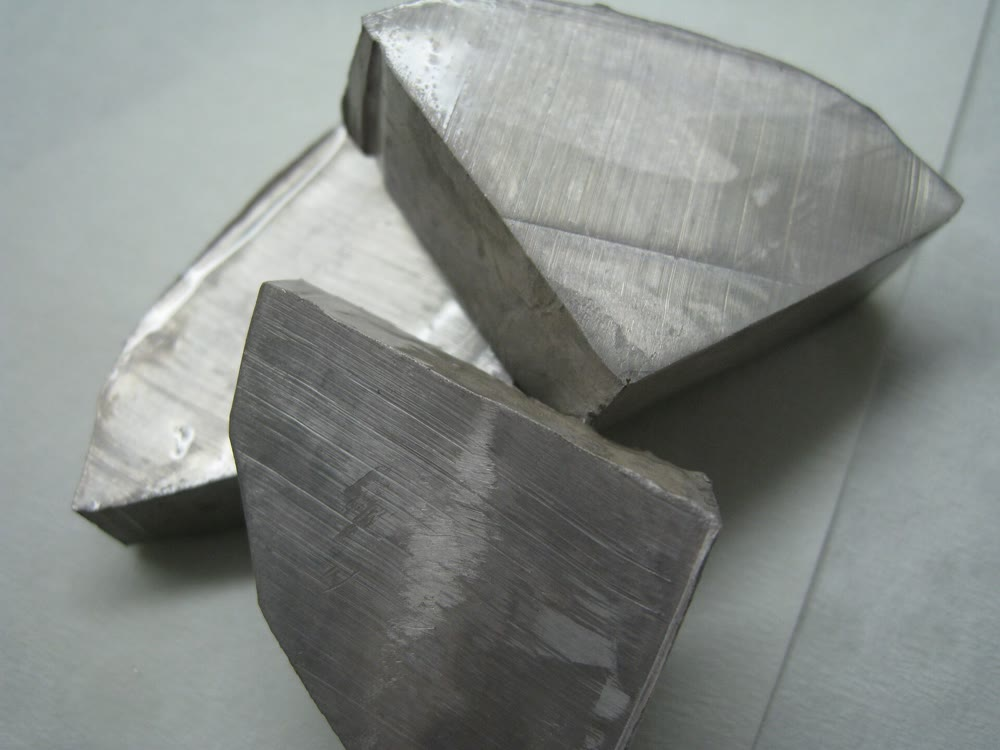
\includegraphics[width=\linewidth,height=4.4cm,keepaspectratio]{images/book1/sodium.jpg}

{\small Sodium, an \omterm{def:g10:electron-shells:family}{alkali metal}, cut with a knife: soft and silvery when
fresh, it dulls at once in \omterm{def:g4:air-a-mixture-of-gases:air}{air}. Photo: Dnn87, CC BY-SA 3.0.}
\end{minipage}\hfill
\begin{minipage}[b]{0.48\linewidth}\centering
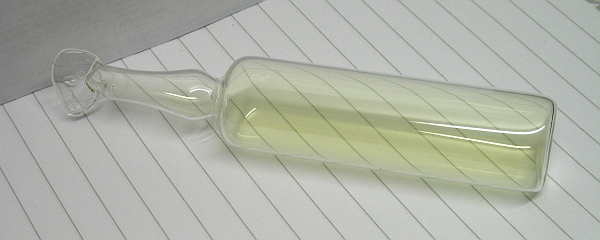
\includegraphics[width=\linewidth,height=4.4cm,keepaspectratio]{images/book1/chlorine-ampoule.jpg}

{\small Chlorine, a \omterm{def:g10:electron-shells:family}{halogen}: a yellow-green gas, here sealed in a glass
ampoule. Photo: W.~Oelen, CC BY-SA 3.0.}
\end{minipage}
\end{omfigure}

\begin{inthelab}[Sodium in water]
Behind a screen, the teacher drops a piece of sodium the size of a grain
of rice into a large bowl of water. It floats, melts into a shiny ball and
whizzes about, fizzing, until it has gone; the gas given off is hydrogen,
and the water left is basic.
\end{inthelab}

\begin{safety}{\ghs[0.75cm]{GHS02}\ghs[0.75cm]{GHS05}\quad\ghs[0.75cm]{GHS03}\ghs[0.75cm]{GHS06}}
% ledger: ghs:Na, ghs:Cl2
Sodium: releases flammable hydrogen with water (GHS02), causes severe
burns (GHS05). Chlorine: an oxidising gas (GHS03), toxic if inhaled
(GHS06), also an irritant and very toxic to aquatic life. Both are
handled only by the teacher.
\end{safety}

\section{Stable ions and the noble-gas rule}

\begin{definition}[Duet and octet rules]\label{def:g10:electron-shells:octet}
The \omterm{def:g10:electron-shells:family}{noble gases}, with a full outer \omterm{def:g10:electron-shells:configuration}{shell}, hardly react: their
configuration is especially stable. When \omterm{def:g7:atoms-and-molecules:atom}{atoms} of the first elements form
\omterm{def:g9:ions:ion}{ions}, they gain or lose \omterm{def:g9:inside-the-atom:nucleus}{electrons} so as to reach the configuration of the
nearest \omterm{def:g10:electron-shells:family}{noble gas}: two \omterm{def:g9:inside-the-atom:nucleus}{electrons} in \omterm{def:g10:electron-shells:configuration}{shell} 1, like helium, for the
lightest \omterm{def:g7:atoms-and-molecules:atom}{atoms} --- the \emph{duet rule}\index{duet rule} --- and eight
\omterm{def:g9:inside-the-atom:nucleus}{electrons} in the outer \omterm{def:g10:electron-shells:configuration}{shell}, like neon or argon, for the others --- the
\emph{octet rule}\index{octet rule}.
\end{definition}

\begin{example}[Ions predicted by the rule]\label{ex:g10:electron-shells:ions}
Sodium, $2.8.1$, loses its single \omterm{def:g10:electron-shells:valence}{valence electron}: \ce{Na+}, $2.8$, like
neon. Magnesium, $2.8.2$, loses two: \ce{Mg^{2+}}. Aluminium, $2.8.3$,
loses three: \ce{Al^{3+}}. Chlorine, $2.8.7$, gains one: \ce{Cl-}, $2.8.8$,
like argon. Oxygen, $2.6$, gains two: \ce{O^{2-}}. Sulfur, $2.8.6$:
\ce{S^{2-}}. Lithium, $2.1$, loses one and keeps $2$, like helium:
\ce{Li+}.
\end{example}

\begin{omfigure}
\begin{tikzpicture}[font=\small]
  \foreach \x/\nm/\cfg/\col in {0/{Na}/{$1\mathrm{s}^2\,2\mathrm{s}^2\,2\mathrm{p}^6\,3\mathrm{s}^1$}/omDef,
      5.8/{\ce{Na+}}/{$1\mathrm{s}^2\,2\mathrm{s}^2\,2\mathrm{p}^6$}/omProp,
      11.0/{Ne}/{$1\mathrm{s}^2\,2\mathrm{s}^2\,2\mathrm{p}^6$}/gray} {
    \node[draw=\col, fill=\col!6, rounded corners=2pt, align=center, text width=3.4cm]
      at (\x,0) {\textbf{\nm}\\ \cfg};
  }
  \draw[->, thick, omProp] (2.0,0) -- (3.8,0) node[midway, above, font=\footnotesize] {loses 1 \ce{e-}};
  \node at (8.4,0) {$=$};
  \node[font=\footnotesize, align=center] at (8.4,-0.75) {same\\ configuration};
\end{tikzpicture}

{\small The sodium \omterm{def:g9:ions:ion}{ion} has the configuration of neon, the nearest \omterm{def:g10:electron-shells:family}{noble
gas}.}
\end{omfigure}

\begin{remark}[Limits of the rule]\label{rem:g10:electron-shells:limits}
The rule works well for the first twenty elements and their simple \omterm{def:g9:ions:ion}{ions}.
Many elements, such as iron (\ce{Fe^{2+}} and \ce{Fe^{3+}}), do not
follow it; the reasons, and a better description of \omterm{def:g9:inside-the-atom:nucleus}{electrons}, are given
in the Year 1 volume.
\end{remark}

\section{Exercises}

\begin{exercise}[$\star$]\label{exo:g10:electron-shells:1}
Write the \omterm{def:g10:electron-shells:configuration}{electron configurations} of carbon ($Z = 6$), nitrogen ($Z = 7$)
and magnesium ($Z = 12$).
\end{exercise}

\begin{exercise}[$\star$]\label{exo:g10:electron-shells:2}
How many \omterm{def:g10:electron-shells:valence}{valence electrons} do carbon, nitrogen and magnesium have?
\end{exercise}

\begin{exercise}[$\star$]\label{exo:g10:electron-shells:3}
In which period and which group is the element of configuration
$1\mathrm{s}^2\,2\mathrm{s}^2\,2\mathrm{p}^6\,3\mathrm{s}^2\,3\mathrm{p}^3$?
\end{exercise}

\begin{exercise}[$\star$]\label{exo:g10:electron-shells:4}
Name the three families of this chapter and give two elements of each.
\end{exercise}

\begin{exercise}[$\star$]\label{exo:g10:electron-shells:5}
State the \omterm{def:g10:electron-shells:octet}{octet rule}.
\end{exercise}

\begin{exercise}[$\star\star$]\label{exo:g10:electron-shells:6}
Using the noble-gas rule, give the \omterm{def:g9:ions:ion}{ion} formed by potassium ($Z = 19$) and
by fluorine ($Z = 9$), with their configurations.
\end{exercise}

\begin{exercise}[$\star\star$]\label{exo:g10:electron-shells:7}
An element has 2 \omterm{def:g9:inside-the-atom:nucleus}{electrons} in its third \omterm{def:g10:electron-shells:configuration}{shell} and its third \omterm{def:g10:electron-shells:configuration}{shell} is its
outer \omterm{def:g10:electron-shells:configuration}{shell}. Give its configuration, its \omterm{def:g9:inside-the-atom:atomic-number}{atomic number} and its name.
\end{exercise}

\begin{exercise}[$\star\star$]\label{exo:g10:electron-shells:8}
Using stable \omterm{def:g9:ions:ion}{ions}, write the formula of the \omterm{def:g9:ions:ionic-compound}{ionic compound} formed by
magnesium and chlorine, then by aluminium and oxygen.
\end{exercise}

\begin{exercise}[$\star\star$]\label{exo:g10:electron-shells:9}
Look at the table of the first twenty elements. Which elements have the
same number of \omterm{def:g10:electron-shells:valence}{valence electrons} as oxygen?
\end{exercise}

\begin{exercise}[$\star\star$]\label{exo:g10:electron-shells:10}
Why does neon, unlike sodium and chlorine, form no \omterm{def:g9:ions:ion}{ions} in \omterm{def:g7:chemical-reactions:reaction}{chemical
reactions}?
\end{exercise}

\begin{exercise}[$\star\star$]\label{exo:g10:electron-shells:11}
The \omterm{def:g9:ions:ion}{ion} \ce{X^{2+}} has the configuration of argon. Find $X$.
\end{exercise}

\begin{exercise}[$\star\star\star$]\label{exo:g10:electron-shells:12}
Helium has 2 \omterm{def:g10:electron-shells:valence}{valence electrons} but sits in \omterm{def:g9:periodic-table-first-look:period}{group} 18, not \omterm{def:g9:periodic-table-first-look:period}{group} 2.
Explain using its configuration.
\end{exercise}

\begin{exercise}[$\star\star\star$]\label{exo:g10:electron-shells:13}
Potassium reacts with water even more violently than sodium. Using the
distance of the \omterm{def:g10:electron-shells:valence}{valence electron} from the \omterm{def:g9:inside-the-atom:nucleus}{nucleus}, suggest why.
\end{exercise}

\begin{exercise}[$\star\star\star$]\label{exo:g10:electron-shells:14}
Give the configurations of \ce{S^{2-}}, \ce{Cl-}, \ce{K+} and
\ce{Ca^{2+}}. What do they have in common?
\end{exercise}

\begin{exercise}[$\star\star\star$]\label{exo:g10:electron-shells:15}
An element of period 3 forms the \omterm{def:g9:ions:ion}{ion} \ce{Y^{3-}}. Find its group, its
configuration and its name.
\end{exercise}

\section{Problem: Ruby, Sapphire and Corundum}

\begin{problem}[{Weekend problem --- the electrons behind a gemstone: from
two configurations to the number of electrons moved in one gram}]
\label{pb:g10:electron-shells:1}
Rubies and sapphires are gem forms of corundum, an \omterm{def:g9:ions:ionic-compound}{ionic compound} of
aluminium and oxygen; a trace of other \omterm{def:g9:periodic-table-first-look:metal}{metals} gives them their colours.
Corundum is hard enough to scratch almost anything, and powdered corundum
is used to polish lenses. Take the mass of a \omterm{def:g9:inside-the-atom:proton}{nucleon} as
\qty{1.67e-27}{kg}; aluminium-27 has 27 \omterm{def:g9:inside-the-atom:proton}{nucleons}, oxygen-16 has 16.

\medskip
\noindent\textbf{Part I --- The \omterm{def:g7:atoms-and-molecules:atom}{atoms}.}
\begin{enumerate}
  \item Give the numbers of \omterm{def:g9:inside-the-atom:proton}{protons} and \omterm{def:g9:inside-the-atom:nucleus}{electrons} of an aluminium \omterm{def:g7:atoms-and-molecules:atom}{atom}
        ($Z = 13$) and of an oxygen \omterm{def:g7:atoms-and-molecules:atom}{atom} ($Z = 8$).
  \item Write their \omterm{def:g10:electron-shells:configuration}{electron configurations}.
  \item How many \omterm{def:g10:electron-shells:valence}{valence electrons} does each have? In which period and
        group is each?
  \item Is aluminium a \omterm{def:g9:periodic-table-first-look:metal}{metal} or a \omterm{def:g9:periodic-table-first-look:metal}{non-metal}? And oxygen?
\end{enumerate}

\medskip
\noindent\textbf{Part II --- The \omterm{def:g9:ions:ion}{ions}.}
\begin{enumerate}[resume]
  \item Using the \omterm{def:g10:electron-shells:octet}{octet rule}, which \omterm{def:g9:ions:ion}{ion} does aluminium form? Write its
        configuration.
  \item Which \omterm{def:g9:ions:ion}{ion} does oxygen form? Write its configuration.
  \item Which \omterm{def:g10:electron-shells:family}{noble gas} has the same configuration as both \omterm{def:g9:ions:ion}{ions}?
  \item How many \omterm{def:g9:inside-the-atom:nucleus}{electrons} does an aluminium \omterm{def:g7:atoms-and-molecules:atom}{atom} lose, and an oxygen \omterm{def:g7:atoms-and-molecules:atom}{atom}
        gain?
\end{enumerate}

\medskip
\noindent\textbf{Part III --- The formula.}
\begin{enumerate}[resume]
  \item Find the formula of corundum, the neutral compound of these \omterm{def:g9:ions:ion}{ions}.
  \item In one formula unit, how many \omterm{def:g9:inside-the-atom:nucleus}{electrons} are lost by the aluminium
        \omterm{def:g7:atoms-and-molecules:atom}{atoms}? Gained by the oxygen \omterm{def:g7:atoms-and-molecules:atom}{atoms}?
  \item Why must these two numbers be equal?
  \item A ruby contains a trace of chromium \omterm{def:g9:ions:ion}{ions} \ce{Cr^{3+}} in place of
        some \ce{Al^{3+}}. Why can a \ce{Cr^{3+}} \omterm{def:g9:ions:ion}{ion} take the place of an
        \ce{Al^{3+}} \omterm{def:g9:ions:ion}{ion} without upsetting the charges?
\end{enumerate}

\medskip
\noindent\textbf{Part IV --- One gram of corundum.}
\begin{enumerate}[resume]
  \item How many \omterm{def:g9:inside-the-atom:proton}{nucleons} are there in one formula unit of corundum?
  \item Compute the mass of one formula unit (\omterm{def:g9:inside-the-atom:nucleus}{electrons} neglected).
  \item How many formula units are there in \qty{1}{g} of corundum?
  \item How many \ce{Al^{3+}} \omterm{def:g9:ions:ion}{ions} and \ce{O^{2-}} \omterm{def:g9:ions:ion}{ions} is that?
  \item Why can the \omterm{def:g9:inside-the-atom:nucleus}{electrons} be neglected in question 14?
  \item How many \omterm{def:g9:inside-the-atom:nucleus}{electrons} were transferred from aluminium to oxygen to
        make \qty{1}{g} of corundum?
\end{enumerate}
\end{problem}
